% HMC Math dept HW template example
% v0.04 by Eric J. Malm, 10 Mar 2005
\documentclass[10pt,a4paper,boxed]{hmcpset}

% set 1-inch margins in the document
% \usepackage[margin=1in]{geometry}
\usepackage{enumerate}
\usepackage{todonotes}
%\usepackage{tikz}
%\usetikzlibrary{positioning}
\usepackage{subfig} % subfigures in figures.	
\usepackage{pgfplots}
\usepackage{amsmath}
\usepackage{amsfonts}
\usepackage{amssymb}

%% work around for subfig and asy environment
\makeatletter
\newsavebox{\sfe@box}
\newenvironment{subfloatenv}[2]{%
\def\sfe@caption{#1}%
\def\sfe@label{#2}%
\setbox\sfe@box\hbox\bgroup\color@setgroup}%
{\color@endgroup\egroup\subfloat[\sfe@caption]%
{\usebox{\sfe@box}\label{\sfe@label}}}
\makeatother

% include this if you want to import graphics files with /includegraphics
\usepackage{graphicx}

\renewcommand*{\familydefault}{\sfdefault}
\newcommand{\vect}[1]{\mathbf{#1}}


%\tikzset{node distance=2cm, inner/.style={draw,circle}, leaf/.style={draw,rectangle}}

\usepackage{hyperref}

% info for header block in upper right hand corner
\name{Lukas Gesing, Patrick Kaster}
\class{MA-INF 4201 - Artificial Life}
\assignment{Exercise Sheet 4}
% \duedate{09/03/2004}

\begin{document}
\begin{problem}[Assignment 24]
\end{problem}
\begin{solution}
    A loop with the double length of the edges needs twice more \emph{msg.forward} blocks
    Each "70" string/message builds one cell. Each "40" string makes a corner/builds a daughter.
    $\Rightarrow$ to double length of the edges, you just need to double the edges you just need to double the number of "70" messages, i.e. each 12 and take the same number of "40" strings.  
\end{solution}

\begin{problem}[Assignment 25]
\end{problem}
\begin{solution}
The reproduction of the \emph{Chou-Reggia}-loop is basically identical to \emph{Langton's loop}, except that in \emph{Chou-Reggia}-loop all sheaths are removed. Instead of the extending arm, a \emph{growth cap} is developed at the tip of the first \emph{msg.forward} blocks. This \emph{growth cap} provides a sense of orientation, replacing the function of the sheaths.

%\begin{figure}[h!]
%	\centering
%	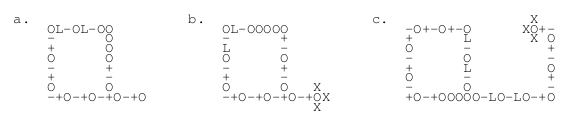
\includegraphics[width=0.8\textwidth]{img/choureggia}
%	\caption{first three steps in replication of a \emph{Chou-Reggia}-loop. From \cite{ChouReggia}. }
%\end{figure}
$t=0:$
\begin{tabular}{|c|c|c|}
\cline{1-2} 
1 & 1 & \multicolumn{1}{c}{}\tabularnewline
\hline 
3 & 4 & 1\tabularnewline
\hline 
\end{tabular}%
$\qquad t=1:$
\begin{tabular}{|c|c|c|}
\cline{1-2} 
1 & 4 & \multicolumn{1}{c}{}\tabularnewline
\hline 
1 & 3 & 5\tabularnewline
\hline 
\end{tabular}%
$\qquad t=2:$
\begin{tabular}{|c|c|c|c}
\cline{1-3} 
4 & 3 & 7 & \tabularnewline
\hline 
1 & 1 & 3 & \multicolumn{1}{c|}{7}\tabularnewline
\hline 
\multicolumn{1}{c}{} &  & 7 & \tabularnewline
\cline{3-3} 
\end{tabular}%\\

$t=3:$
\begin{tabular}{|c|c|c|c|}
\hline 
3 & 1 & 7 & 7\tabularnewline
\hline 
4 & 1 & 1 & 2\tabularnewline
\hline 
\multicolumn{1}{c}{} &  & 7 & 7\tabularnewline
\cline{3-4} 
\end{tabular}%
$\qquad t=4:$
\begin{tabular}{|c|c|c|c|}
\cline{1-2} 
1 & 1 & \multicolumn{1}{c}{} & \multicolumn{1}{c}{}\tabularnewline
\hline 
3 & 4 & 1 & 1\tabularnewline
\hline 
\end{tabular}

\end{solution}

\begin{problem}[Assignment 26]
\end{problem}
\begin{solution}
loop generation $1:$
\begin{tabular}{ccc}
 & $\cdot$ & \tabularnewline
\cline{2-2} 
\multicolumn{1}{c|}{$\cdot$} & \multicolumn{1}{c|}{} & $\cdot$\tabularnewline
\cline{2-2} 
 & $\cdot$ & \tabularnewline
\end{tabular}
$\qquad$ loop generation $2:$
\begin{tabular}{cccc}
 & $\cdot$ & $\cdot$ & \tabularnewline
\cline{2-3} 
\multicolumn{1}{c|}{$\cdot$} & \multicolumn{1}{c|}{} & \multicolumn{1}{c|}{} & $\cdot$\tabularnewline
\cline{2-3} 
 & $\cdot$ & $\cdot$ & \tabularnewline
\end{tabular}

Langton's loop reproduces itself in every direction. It is operating in a $2D$ grid. The structure is growing with the same speed in two dimensions.
First generation loop can grow into four room directions. Second generation loop can only grow into three room directions.
$\Rightarrow$ the space requirement lies somewhere in the magnitude of $\Theta \left( n^2 \right)$.
\end{solution}

\begin{problem}[Assignment 27]
\end{problem}
\begin{solution}
Define:
\begin{align*}
	C(t) & = \mbox{number of symbols C at timestep t} \\
	A(t) & = \mbox{number of symbols A at timestep t} \\
	N(t) & = C(t)+A(t) \mbox{(length f the string)}
\end{align*}

First: Check starting conditions
\begin{align*}
	N(0) & \overset{\mbox{def.}}{=} C(0) + A(0) = 1+0 = 1 \\
	N(1) & \overset{\mbox{def.}}{=} C(1) + A(1) \overset{(1)(2)}{=} A(0)+C(0)+A(0) \\
		 & \overset{\mbox{Axiom}}{=} 0+1+0 = 1
\end{align*}

So for $t=2$ we get:
\begin{align*}
	N(t+1) & \overset{\mbox{def.}}{=} C(t+1) + A(t+1) \\
		   & \overset{(1)(2)}{=} A(t) + C(t) + A(t) \\
		   & \overset{\mbox{def.}}{=} N(t) + C(t-1) + A(t-1) \\
		   & \overset{(2), \mbox{def.}}{=} N(t) + N(t-1) 
\end{align*}

Where in the above we used:

\begin{tabular}{ll}
$(1)$: & How are 'C's produced? Only with rule $2 \Rightarrow C(t+1)=A(t)$ \\ 
$(2)$: & How are 'A's produced? With rule 1 and rule 2: $A(t+1)=C(t)+A(t)$ \\ 
\end{tabular} 
 \end{solution}

\begin{problem}[Assignment 28]
\end{problem}
\begin{solution}
	\begin{tabular}{ll}
	 variables: & R, S, T\\ 
	 axiom: & R \\
	 		& \\
	 rule 1: & $R \rightarrow RS$ \\
	 rule 2: & $S \rightarrow ST$ \\
	 rule 3: & $T \rightarrow TR$ \\
	\end{tabular}
\end{solution}

\newpage

\begin{problem}[Assignment 29]
\end{problem}
\begin{solution}
	\begin{enumerate}[a)]
		\item 
			The $B \rightarrow B C$ rule adds one unit length per turn, thus controls the length of the segments. The $A \rightarrow A +B C +B C$ concatenates the turns of the spiral.
			%\begin{table}[h!]
				\begin{tabular}[t]{ll}
					 variables: & A, B, C\\ 
					 constants: & +,- \\
					 axiom: & -A \\
							& \\
					 rule 1: & $A \rightarrow A +B C +B C$ \\
					 rule 2: & $B \rightarrow B C$ \\
				\end{tabular}
			%\end{table}

		\item 
			%\begin{table}[h!]
				\begin{tabular}[t]{ll}
					 variables: & B, C, D, E, F\\ 
					 constants: & +,- \\
					 axiom: & B \\
						    & \\
					 rule 1: & $B \rightarrow C [-B] E [+B]$ \\
					 rule 2: & $C \rightarrow F[-D]F$ \\
					 rule 3: & $F \rightarrow FF$
				\end{tabular}
		\item
				\begin{tabular}[t]{ll}
					 variables: & 0, 1, X\\ 
					 constants: & \\
					 axiom: & X \\
									& \\
					 rule 1: & $X \rightarrow 0000$ \\
					 rule 2: & $0000 \rightarrow 0001$ \\
					 rule 3: & $0001 \rightarrow 0011$ \\
					 rule 4: & $0011 \rightarrow 0010$ \\
					  \vdots & \vdots \\
					 rule 16: & $1001 \rightarrow 1000$ \\
					 rule 17: & $1000 \rightarrow 0000$
				\end{tabular}
			%\end{table}
			more than one symbol $\Rightarrow$ context dependent
	\end{enumerate}
	\begin{figure}[h]
		\centering
		\begin{subfloatenv}{spiral for $\alpha=12^\circ$, $100$ iterations}{fig:spiral}
			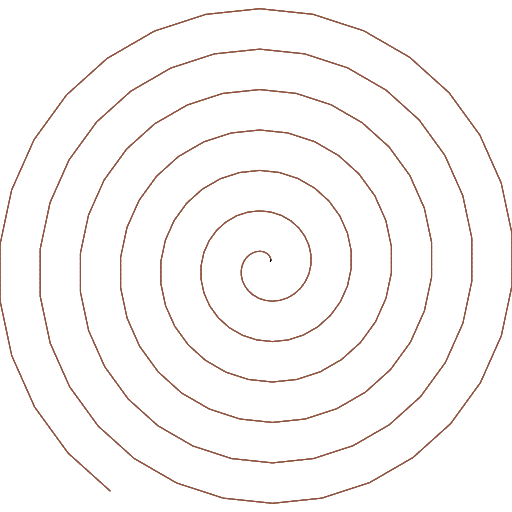
\includegraphics[width=0.3\textwidth]{img/spiral}
		\end{subfloatenv}
		\begin{subfloatenv}{tree, for $\alpha=30^\circ$, $5$ iterations}{fig:tree}
			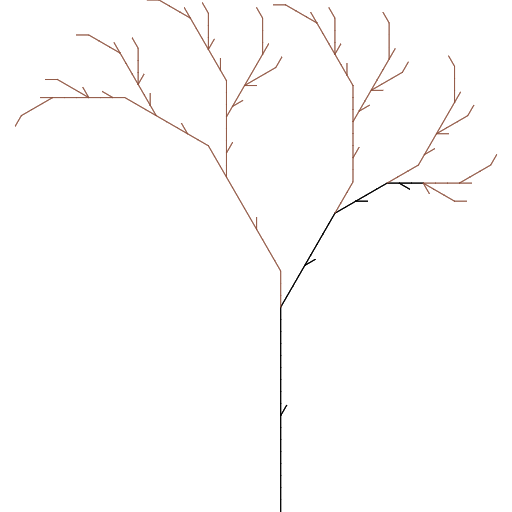
\includegraphics[width=0.3\textwidth]{img/tree}
		\end{subfloatenv}
		%\caption{proof by induction over points on a circle}
			% das label muss immer nach der caption kommen, sonst gibt es Probleme bei der Referenzierung und Nummerierung.
		\label{fig:plots}
	\end{figure}
\end{solution}

\pagebreak

%\begin{problem}[Assignment 30]
%\end{problem}
%\begin{solution}
%\end{solution}

\begin{thebibliography}{[01]}
\bibitem[01]{ChouReggia} Reggia, James A and Chou, Hui-Hsien and Lohn, Jason D: "Cellular automata models of self-replicating systems" published in "Advances in Computers", volume 47, pp. 141--183, \emph{Elsevier}, 1998

\end{thebibliography}

\end{document}
